\documentclass[11pt]{article}

%%METADATA
\title{GA1025 Macro Theory \\Solution to Problem Set 6}
\author{
Junbiao Chen\thanks{E-mail: jc14076@nyu.edu.}
}
\date{\today}


%%PACKAGES
\usepackage{mdframed} % For boxed environments
\usepackage{graphicx}
\usepackage{grffile}
\usepackage{tabularx}
\usepackage{setspace}
\usepackage{amsmath,amsthm,amssymb}
\usepackage[hyphens]{url}
\usepackage{natbib}
\usepackage[font=normalsize,labelfont=bf]{caption}
\usepackage[margin=1in]{geometry}
\usepackage{hyperref}
\hypersetup{colorlinks=true,urlcolor=blue,citecolor=blue}
\usepackage{stmaryrd}  %Package with \boxast command
\usepackage{enumerate}% http://ctan.org/pkg/enumerate %Supports lowercase Roman-letter enumeration
\usepackage{verbatim} %Package with \begin{comment} environment
%\usepackage{enumitem}
\usepackage{physics}
\usepackage{tikz}
\usepackage{listings}
\usepackage{upquote}
\usepackage{booktabs} %Package with \toprule and \bottomrule
\usepackage{etoc}     %Package with \localtableofcontents
\usepackage{placeins}    %Package that prevent repositioning the tables
\usepackage{multicol}
\usepackage{bm}
\usepackage{subfig}
\usepackage{csquotes}

\definecolor{dkgreen}{rgb}{0,0.6,0}
\definecolor{gray}{rgb}{0.5,0.5,0.5}
\definecolor{mauve}{rgb}{0.58,0,0.82}

\lstset{language=bash,
  frame=tb,
  aboveskip=3mm,
  belowskip=3mm,
  showstringspaces=false,
  columns=flexible,
  basicstyle={\small\ttfamily},
  numbers=none,
  numberstyle=\tiny\color{gray},
  keywordstyle=\color{blue},
  commentstyle=\color{dkgreen},
  stringstyle=\color{mauve},
  breaklines=true,
  breakatwhitespace=false,
  tabsize=3
}

\lstset{language=C,
  aboveskip=3mm,
  belowskip=3mm,
  showstringspaces=false,
  columns=flexible,
  basicstyle={\small\ttfamily},
  numbers=none,
  numberstyle=\tiny\color{gray},
  keywordstyle=\color{blue},
  commentstyle=\color{dkgreen},
  stringstyle=\color{mauve},
  breaklines=true,
  breakatwhitespace=false,
  tabsize=4
}

\definecolor{lightblue}{rgb}{0.68, 0.85, 0.9} %

%CUSTOM DEFINITIONS
\theoremstyle{definition}
\newtheorem{definition}{Definition}[section]
\newtheorem*{remark}{Remark}
\setcounter{secnumdepth}{3}
\usepackage{tikz}
\usetikzlibrary{arrows.meta}
\usetikzlibrary{automata, positioning, arrows, calc}

\tikzset{
	->,  % makes the edges directed
	>=stealth, % makes the arrow heads bold
	shorten >=2pt, shorten <=2pt, % shorten the arrow
	node distance=3cm, % specifies the minimum distance between two nodes. Change if n
	every state/.style={draw=blue!55,very thick,fill=blue!20}, % sets the properties for each ’state’ n
	initial text=$ $, % sets the text that appears on the start arrow
 }

%% PROPOSITION
% Define the Proposition environment
\newmdenv[
  innerleftmargin=10pt, 
  innerrightmargin=10pt,
  innertopmargin=10pt,
  innerbottommargin=10pt,
  linecolor=black, 
  linewidth=1pt,
  backgroundcolor=white, 
  roundcorner=5pt
]{propositionbox}

\newtheoremstyle{boldtitle} % Define a new theorem style
  {10pt} % Space above
  {10pt} % Space below
  {\itshape} % Body font
  {} % Indent amount
  {\bfseries} % Theorem head font
  {.} % Punctuation after theorem head
  { } % Space after theorem head
  {} % Theorem head spec

\theoremstyle{boldtitle} % Use the custom style
\newtheorem{proposition}{Proposition} % Define the proposition environment

% Redefine the proposition environment to use the box
\newenvironment{boxedproposition}[1][]
{\begin{propositionbox}\begin{proposition}[#1]}
{\end{proposition}\end{propositionbox}}

%%FORMATTING
\usepackage[bottom]{footmisc}
\onehalfspacing
\numberwithin{equation}{section}
\numberwithin{figure}{section}
\numberwithin{table}{section}
\bibliographystyle{../bib/aeanobold-oxford}


%main text
\begin{document}

\maketitle


\section{Permanent income model}
The household maximizes the present value of utility from consumption
\[
E_0 \left[ \sum_{t=0}^\infty \beta^t u(c_t) \right]
\]
where $\beta \in (0,1)$ and $u(c) = -\frac{1}{2}(c - c^*)^2$ is a quadratic utility function. The consumer chooses a plan for consumption and borrowing $\{c_t, b_{t+1}\}_{t=0}^\infty$ subject to a sequence of budget constraints
\[
c_t + b_t = R^{-1} b_{t+1} + y_t
\]
and a no-Ponzi scheme restriction
\[
E_0 \left[ \sum_{t=0}^\infty \beta^t b_t^2 \right] < \infty.
\]

The exogenous income process satisfies $y_t = z_{1,t} + z_{2,t}$ with $z_t = (z_{1,t}, z_{2,t})'$ given by
\[
\begin{bmatrix}
z_{1,t+1} \\
z_{2,t+1}
\end{bmatrix}
=
\begin{bmatrix}
\rho_1 & 0 \\
0 & \rho_2
\end{bmatrix}
\begin{bmatrix}
z_{1,t} \\
z_{2,t}
\end{bmatrix}
+
\begin{bmatrix}
\sigma_1 & 0 \\
0 & \sigma_2
\end{bmatrix}
\begin{bmatrix}
w_{1,t+1} \\
w_{2,t+1}
\end{bmatrix}
\]
where $w_{t+1} \sim N(0, I_2)$ is an i.i.d. shock.

We consider two information structures. In the full information case, the household observes components of $z_t$ and hence the structural shocks $w_{1,t}$ and $w_{2,t}$. In the incomplete information case, the household only observes income $y_t$ and needs to filter the contribution of both income components $z_{1,t}$ and $z_{2,t}$ to income.

\textbf{Question 1:}
$\rho_1 = \rho$ and $\rho_2 = 0$. 
Find analytical expressions for the impulse responses of consumption and debt 
to unit shocks $w_{1,t}$ and $w_{2,t}$ in the full information case, 
and to a unit innovation in income in the incomplete information case.

\subsection*{Solution to Q1}
Following the derivation in the lecture note, we can express this linear quadratic permanent income model in the following state space:
\begin{align*}
    z_{t+1} & = A_{22} z_t + C_2 w_t \\
    y_t & = U_y z_t \\ 
    b_{t+1} &= b_t - U_y \left(I - \beta A_{22} \right)^{-1} \left( I - A_{22}\right) z_t \\
    c_t &= (1 - \beta) \left(U_y (I - \beta A_{22})^{-1} z_t - b_t \right)
\end{align*}
where 
\[
z_{t+1} = \begin{bmatrix}
z_{1,t+1} \\
z_{2,t+1} 
\end{bmatrix}, \quad 
A_{22} = \begin{bmatrix}
\rho_1 & 0 \\
0 & \rho_2
\end{bmatrix}, \quad 
C_2 = \begin{bmatrix}
\sigma_1 & 0 \\
0 & \sigma_2
\end{bmatrix}, \quad 
U_y = \begin{bmatrix}
1 & 1
\end{bmatrix}
\]

Define $A_{12} = - U_y \left(I - \beta A_{22} \right)^{-1} \left( I - A_{22}\right)$, 
we have 
\begin{align*}
    h_t(b) & = A_{12} \left( I - A_{22}^{t} \right) \left( I - A_{22} \right)^{-1} C_2 \\ 
        & =  - U_y \left(I - \beta A_{22} \right)^{-1} \left( I - A_{22}^{t} \right) C_2 \\
        & = - \begin{bmatrix} 1 & 1 \end{bmatrix} \begin{bmatrix} \frac{1}{1 - \beta \rho} & 0 \\ 0 & 1 \end{bmatrix} \begin{bmatrix} 1 - \rho^t & 0 \\ 0 & 1 \end{bmatrix} \begin{bmatrix} \sigma_1 & 0 \\ 0 & \sigma_2 \end{bmatrix} \\ 
        & = - \begin{bmatrix} \sigma_1 \left( \frac{1 - \rho^t}{1 - \beta \rho} \right) & \sigma_2 \end{bmatrix}
\end{align*}

After similar derivation, the impulse response for consumption is given by 
\begin{align*}
h_t(c) & = (1 - \beta) U_y \left(I - \beta A_{22} \right)^{-1} C_2 \\
& =  [\begin{matrix} (1 - \beta) & (1 - \beta) \end{matrix}] \left[\begin{matrix} \frac{1}{1 - \beta \rho} & 0 \\ 0 & 1 \end{matrix} \right] \left[\begin{matrix} \sigma_1 & 0 \\ 0 & \sigma_2 \end{matrix} \right] \\ 
& = \begin{bmatrix} \left(\frac{1 - \beta}{1 - \beta \rho} \right)\sigma_1 & (1-\beta)\sigma_2 \end{bmatrix}
\end{align*}

Given $\rho = 0.5, \beta = 0.95, \sigma_1 = \sigma_2 =1$, 
the impulse responses of debt to unit shocks $w_{1,t}$ and $w_{2,t}$ are given by:
\begin{align*}
    \tilde{b}_{t+1} - b_{t+1} & = - \sigma_1 \left( \frac{1 - \rho^t}{1 - \beta \rho} \right)  \\
    \tilde{b}_{t+1} - b_{t+1} & = - \sigma_2,
\end{align*}
respectively.

\begin{figure}[htbp]
  \centering
  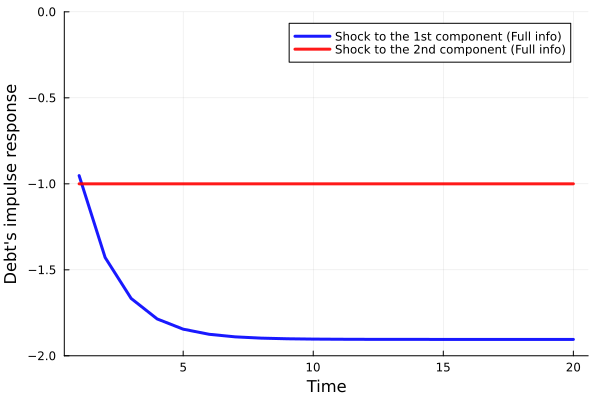
\includegraphics[width=0.45\textwidth]{images/debt_impulse_response_functions.png}
  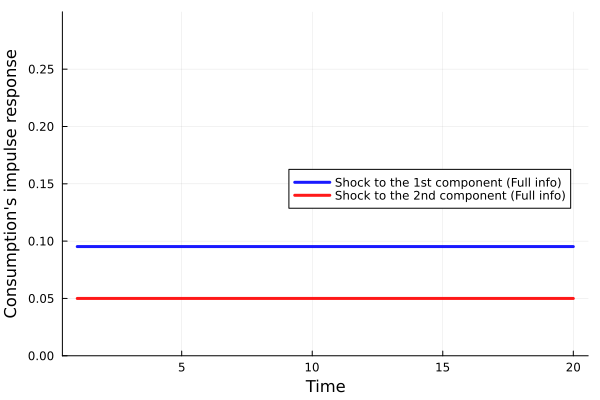
\includegraphics[width=0.45\textwidth]{images/consumption_impulse_response_functions.png}
  \caption{Impulse Responses}
\end{figure}


In a setting with unobservable states, 
the agent needs to apply ``Kalman Filter'' to obtain information from the data.
Since $z_{2,t}$ represents the transitory shock, 
the system is given by the following state-space representation:
\begin{align*}
    a_t & = y_t - \hat{z}_{1, t} = y_t - E[y_t | y^{t-1}] \\
    K_1 & = \frac{\Sigma_{11}}{\Sigma_{11} + \Sigma_{22}} \\ 
    \hat{z}_{1, t+1} & = \rho \hat{z}_{1, t} + K_1 a_t \\ 
    \hat{z}_{2, t+1} & = 0 \\ 
    \Sigma & =   \left[ \begin{matrix}
        \Sigma_{11} & 0 \\ 0 & \Sigma_{22}
    \end{matrix}  \right], \quad  \Sigma_{11}  = \frac{K_1^2 \sigma_2^2 + \sigma_1^2}{1 - (1 - K)^2}, \quad  \Sigma_{22} = \sigma_2^2 
\end{align*} 
Since the agent cannot observe the shocks directly, 
I formulate the problem using ``the innovation'' from the Kalman filter ($a_t$) and 
the observed data ($y_t$) as states.
\begin{align*} 
    \begin{bmatrix} y_{t+1} \\ a_{t+1} \end{bmatrix} & = 
    \begin{bmatrix} \rho & K_1 - \rho \\ 0 & 0 \end{bmatrix} \begin{bmatrix} y_t \\ a_t \end{bmatrix} + \begin{bmatrix} 1 \\ 1 \end{bmatrix} a_{t+1} \\
    y_t & = \begin{bmatrix} 1 & 0 \end{bmatrix}  \begin{bmatrix} y_t \\ a_t \end{bmatrix}  
\end{align*}
Define 
\[
\tilde{A}_{22} = \begin{bmatrix} \rho & K_1 - \rho \\ 0 & 0 \end{bmatrix}  
\]
Then, following the derivation under the complete information structure, we have 
\[
h_t(c) = \begin{bmatrix} (1 - \beta) & 0 \end{bmatrix}  
         \begin{bmatrix} \frac{1}{1 - \beta \rho} & \frac{\beta (K_1 - \rho)}{1 - \beta \rho} \\ 0 & 0 \end{bmatrix} 
         \begin{bmatrix} 1 \\ 1 \end{bmatrix}
        = \frac{(1 - \beta) \left[1 + \beta (K_1 - \rho)\right]}{1 - \beta \rho}
\]
Similarily, we have 
\begin{align*}
h_t(b) & = - \tilde{U}_y \left(I - \beta \tilde{A}_{22} \right)^{-1} \left( I - \tilde{A}_{22}^t \right) \tilde{C}_2 \\ 
    & = - \begin{bmatrix} 1 & 0 \end{bmatrix} 
    \begin{bmatrix} \frac{1}{1 - \beta \rho} & \frac{\beta (K_1 - \rho)}{1 - \beta \rho} \\ 0 & 1 \end{bmatrix} 
    \begin{bmatrix} (1 - \rho^t) & \quad - \rho^{t-1} (K_1 - \rho) \\ 0 & 1 \end{bmatrix} 
    \begin{bmatrix} 1 \\ 1 \end{bmatrix} \\ 
    & = - \bm{1}_{t \geq 1} \left(1 + \frac{K_1 \left( \beta - \rho^{t-1} \right)}{1 - \beta \rho} \right)
\end{align*}

% \begin{enumerate}

% \item 

%     Plot the impulse responses for the case $\rho = 0.5$, $\beta = 0.95$, $\sigma_1 = \sigma_2 = 1$.

% \item As $\rho \to 1$, do the impulse responses in the full information model associated with the persistent shock converge to those obtained for the case $\rho = 1$? Explain the economic mechanism.

% \item Derive equations that the solution for general values $\rho_1$ and $\rho_2$ must satisfy. Plot the impulse responses for the case $\rho_1 = 0.99$, $\rho_2 = 0.5$, $\beta = 0.95$, $\sigma_1 = \sigma_2 = 1$.

% \end{enumerate}

\paragraph{Solution to Q2}
As $rho$ increases, the persistency of a positive income shock lasts longer.
Hence, we see the impulse response function shifts downward for each period. 
\begin{figure}[htbp]
  \centering
  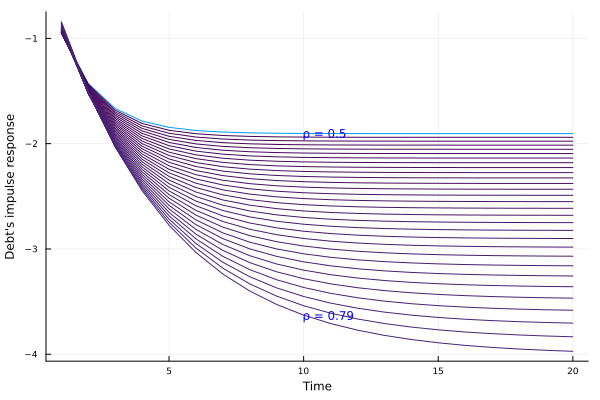
\includegraphics[width=0.45\textwidth]{images/convergence_of_debt_impulse_response_functions.png}
  \caption{Impulse Responses}
\end{figure}

\subsection*{Solution to Q3}
Following the derivation in the lecture note, we can express this linear quadratic permanent income model in the following state space:
\begin{align*}
    z_{t+1} & = A_{22} z_t + C_2 w_t \\
    y_t & = U_y z_t \\ 
    b_{t+1} &= b_t - U_y \left(I - \beta A_{22} \right)^{-1} \left( I - A_{22}\right) z_t \\
    c_t &= (1 - \beta) \left(U_y (I - \beta A_{22})^{-1} z_t - b_t \right)
\end{align*}

\section{Learning about match quality}
\paragraph{Solution to Problem 2.1}
The Kalman filter characterization of the problem is given by 
\begin{align*}
    a_t & = y_t - m_{t-1} \\ 
    K_t & = \frac{\Sigma_t}{\Sigma_t + R} \\ 
    m_t & = m_{t-1} + K_t a_t = (1 - K_t) a_t + K_t y_t \\ 
    \Sigma_{t+1} = \frac{\Sigma_t R}{\Sigma_t + R}
\end{align*}

\paragraph{Solution to Question 2.2}
As the true productivity (match quality) is revealed at $T+1$, the worker will earn $\theta$ forever if she chooses to stay.
Note that she won't leave in the future if she chooses to stay at $T+1$ because the outside option remains the same.
Since the worker won't receive any wage income if she chooses to leave, the Bellman equation is given by 
\begin{align*}
v_{T+1} = \max_{\{\text{Stay, leave}\}} \bigg\{ \frac{\theta}{1 - \beta}, \beta Q \bigg\},
\end{align*}
where $Q$ is the beginning-of-period value of joining a new firm.

\paragraph{Solution to Question 2.3}
Since both the firm and the worker predict the distribution of match quality in the future based on the new information,
we can formulate the the following Bellman equation 
\[
V_{T}(m_T) = \max_{\{\text{Stay, leave} \}} \bigg\{m_T + \beta \int V_{T+1}(\theta) dF(\theta | m_T, \Sigma_{T+1}) d\theta , \beta Q \bigg\}
\]

\paragraph{Solution to Question 2.4}
Continuing backward, we can write down the Bellman equation as follows
\[
V_{t-1}(m) = \max_{\{\text{Stay, leave} \}} \bigg\{m + \beta \int V_{t}(\theta) dF(\theta | m, K_t\Sigma_{t}) d\theta , \beta Q \bigg\}
\]

\paragraph{Solution to Question 2.5}
The ex ante value of the job $Q$ right before $y_0$ has been observed is given by 
\[
Q = \int V_0(m) dF(m|\mu, K_0\Sigma_0)d\theta 
\]

\paragraph{Solution to Question 2.6}
At $t=T$, the reservation wage is given by $\bar{w}_T = (1- \beta)\beta Q$.
\\
At $t=T-1$, the reservation wage is given
\[
\bar{w}_t = \beta \left( Q - \int V_{t+1}(\theta)dF(\theta| m_t, K_t\Sigma_t) d\theta \right)
\]

\paragraph{Solution to Question 2.7}
We can apply an iterative algorithm with damping parameters:
\\
\noindent For iteration $j$
\begin{enumerate}
    \item Guess: $Q(j)$
    \item Compute $V_T(j) = \max \{\frac{\theta}{1 - \beta}, \beta Q(j) \}$
    \item Solve for $V_0$ using backward induction.
    \item Compute the implied new-jobg value $Q$ according to 
    \begin{align*}
        Q(j)^{\text{implied}} = \int V_0(m) dF(m|\mu, K_0\Sigma_0)d\theta 
    \end{align*}
    \item Update the guess for $Q$ according to $Q(j+1) = 0.9 Q(j) + 0.1 \times Q(j)^{\text{implied}}$
    \item Iterate till convergence in terms of $Q$.
\end{enumerate}

\section{Value functions and consumption growth}
\subsection*{Solution to Question 3.1}
The Bellman equation is given by 
\[
V(c_t, g_t) = u(c_t) + \beta \sum_{j} \mathbb{P}\left( g_{t+1} = g_j | g_t \right) V(g_j c_t, g_j),
\]
where $c_t$ and $g_t$ are currect level of consumption and the previous growth rate, respectively.

\subsection*{Solution to Question 3.2}
Guess: $V(c, g) = u(c)w(g)$ and plug it in the Bellman equation above, then we have
\[
u(c)w(g) = u(c) + \beta \sum_{j} \mathbb{P}\left( g' = g_j | g \right) u(g_jc) w(g_j)
\]
Given $u(c) = \frac{c^{1 - \gamma}}{1 - \gamma}$, and denote $w(g_i) = w_i$, we have 
\[
\frac{c^{1 - \gamma}}{1 - \gamma} w_i = \frac{c^{1 - \gamma}}{1 - \gamma} + \beta \sum_j \mathbb{P}_{ij} \frac{(g_jc)^{1 - \gamma}}{1 - \gamma} w_j 
\]
Deviding both sides by $\frac{c^{1 - \gamma}}{1 - \gamma}$, we have 
\[
w_i = 1 + \beta \sum_j \mathbb{P}_{ij}(g_j)^{1 - \gamma} w_j.
\]

\subsection*{Solution to Question 3.3}
Note that we can express $w_i = 1 + \beta \sum_j \mathbb{P}_{ij}(g_j)^{1 - \gamma} w_j$ in the following matrix form:
\[
w = \bm{1}_n + \beta \mathbb{P} \text{diag}(g^{1-\gamma}) w,
\]
where 
\[
\text{diag}(g^{1-\gamma}) = \begin{bmatrix}
    g_1^{1-\gamma} & 0 & \dots & 0 \\ 
    0 & g_2^{1-\gamma} & \dots & 0 \\ 
    \vdots & & \dots & \vdots \\
    0 & 0 & \dots & g_n^{1-\gamma} 
\end{bmatrix}.
\]
Therefore, 
\[
w = \left( I - \beta \mathbb{P}\text{diag}(g^{1-\gamma})\right)^{-1}
\]
As a result, $v^* < \infty$ if $ \left( I - \beta \mathbb{P}\text{diag}(g^{1-\gamma})\right)^{-1}$ is stable.


\subsection*{Solution to Question 3.4}
Using the guess that $V(c, g) = \log c + v(g)$, the preference recursion becomes 
\[
\log c_t + v(g_t) = (1 - \beta) \log c_t + 
\beta \frac{2}{\sigma} \log \mathbb{E}_t \left[ \exp \left(\frac{\sigma}{2} (\log c_{t+1} + v(g_{t+1})) \right) \right]
\]
After simplification, we have 
\[
v(g_t) = \frac{2\beta}{\sigma} \log \mathbb{E}_t \bigg[g_{t+1}^{\sigma/2} \exp(\frac{\sigma}{2}v(g_{t+1})) \bigg],
\]
which can be solved via Value Function Iteration.
\section{Industry equilibrium with investment}
\subsection*{Answer to question 4.1}
The sequence problem for the firm at time $t = 0$ is given by 
\begin{align*}
v^* = \max_{k_{t+1}, k_t} \quad &  \sum_{t=0}^{\infty} \beta^t R_t \\ 
    \text{subject to } \quad k_{t+1} & = (1 - \delta)k_t + i_t \\ 
    y_t & = A k_t \\ 
    y_t & = i_t + s_t \\ 
    \text{given } & k_0 \\ 
    & p_t = \alpha_0 - \alpha_1 S_t, \quad \alpha_0, \alpha_1 > 0 \\
    & S_{t+1} = H_0 + H_1 S_t
\end{align*}

\subsection*{Answer to question 4.2}
After plugging in the budget constraint, the sequence problem becomes 
\[
v^* = \max_{k_{t+1}} \sum_{t=0}^{\infty} \beta^t 
    \bigg\{ (\alpha_0 - \alpha_1 S_t) [(A+1 - \delta) k_t - k_{t+1}] - \frac{b}{2}(k_{t+1} - k_t)^2
    \bigg\}
\]
\noindent F.O.C are given by 
\begin{align*}
    [k_{t+1}] \quad & - \beta^t \bigg[(\alpha_0 - \alpha_1 S_t) - b(k_{t+1} - k_t) \bigg]+ \beta^{t+1} \bigg[ (\alpha_0 - \alpha_1 S_{t+1}) \left[(A+1 -\delta) + b(k_{t+2} - k_{t+1})\right]\bigg] = 0
\end{align*}
After simplications, the optimal conditions are given by 
\begin{align*}
    & \alpha_0 - \alpha_1 S_t + b(k_{t+1} - k_t)  =  \beta \bigg[(\alpha_0 - \alpha_1 S_{t+1}) (A+1 -\delta) + b(k_{t+2} - k_{t+1})\bigg]
\end{align*}
% We also need the transversality condition to complete the optimality conditions:
% \[
% \lim_{t\rightarrow \infty} \beta^t v_k(k) = 0
% \]
\subsection*{Answer to question 4.3}
The specification follows the struture of the ``little-k-big-K'' problem.
As $s = y - i = Ak - (k' - (1 - \delta)k)$, 
the recursive form of the firm's problem is given by
\begin{equation}
    \label{eqn:equilibrium_firm_bellman}
    \begin{aligned}
        & v(k, S) = \max_{k'} \quad (\alpha_0 - \alpha_1 S) \bigg[(A + 1 - \delta)k - k'\bigg] - \frac{b}{2} \left(k' - k \right)^2 + \beta v(k', S') \\
        \text{subject to } \quad & S' = H_0 + H_1 S
    \end{aligned}
\end{equation}


\subsection*{Answer to question 4.4}
The first order conditions are 
\begin{align*}
[k']&: \quad (\alpha_0 - \alpha_1 S) + b (k' - k) = \beta V_k (k', S')\\ 
\text{(By Envelope Theorem) } \quad [k]&: V_k(k, S) = (\alpha_0 - \alpha_1 S) (A + 1 - \delta) + b(k' - k)
\end{align*}
Combining these two conditions together, we have 
\[
(\alpha_0 - \alpha_1 S) + b (k' - k) = \beta \bigg[  (\alpha_0 - \alpha_1 S') (A + 1 - \delta) + b(k''- k')\bigg]
\]
Notice that we require the optimal path in the original sequence problem satisfies the transversality condition:
\[
\lim_{t\rightarrow \infty} \beta^t v_k(k, S)k = 0
\]

\subsection*{Answer to question 4.5}
Denote the optimal policy of the \textbf{representative} firm by $k_{t+1} = h(k_t, S_t)$.
The recursive competitive equilibrium of the model is given by 
a value function $V(k, S)$, an optimal policy function $h(k, S)$, and an aggregate law of motion $H(S)$,
such that 
\begin{enumerate}
    \item Given $H$, $V(k, S)$ satisfies the firm's Bellman equation and optimal policy fuction in (\ref{eqn:equilibrium_firm_bellman});
    \item The law of motion $H$ satisfies $H(S) = h(S, S)$.
\end{enumerate}

\subsection*{Answer to questions 4.6 and 4.7}
To solve for the unique capital level, I recast the model in terms of the state of $K$.
I can do so by replacing $S$ with $K$ and $K'$ because
\[
S = Y - I = AK - (K' - (1 - \delta)K)
\]

I construct the following planner problem:
\[
V(K) = \max_{K'} \quad \alpha_0 \bigg[(A+1 -\delta)K - K' \bigg] - \alpha_1 \bigg[(A+1 -\delta)K - K' \bigg]^2 - \frac{b}{2}(K' - K)^2 + \beta V(K')
\]
It follows that the Euler equation and the Envelope Conditions are 
\begin{align*}
    &  \beta V_K(K') = b(K' - K) + \alpha_0 - 2 \alpha_1 \bigg((A + 1 - \delta)K - K' \bigg) \\ 
    &  V_K(K) = \alpha_0 (A + 1 - \delta) - 2 \alpha_1 \bigg((A + 1 - \delta)K - K' \bigg)(A + 1 - \delta) + b(K'-K)
\end{align*}
Combining these two, we have 
\[
b(K' - K) + \alpha_0 - 2 \alpha_1 \bigg((A + 1 - \delta)K - K' \bigg) = \beta \bigg[ \alpha_0 (A + 1 - \delta) - 2 \alpha_1 \bigg((A + 1 - \delta)K' - K'' \bigg)(A+1 - \delta) + b(K''-K')\bigg]
\]
After collecting terms, we have 
\begin{align*}
0 = \alpha_0 & - \beta \alpha_0 (A+1 - \delta) \\ 
    & - \left[ b + 2 \alpha_1 (A+1 - \delta) \right]K_t \\ 
    & + \left[ b + 2 \alpha_1 + 2 \alpha_1 \beta (A+1 - \delta)^2 + b \beta \right]K_{t+1} \\ 
    & - \left[ \beta b + 2 \alpha_1 \beta (A+1 - \delta) \right]K_{t+2} 
\end{align*}
It follows that
\begin{align*}
K_{t+2}
    - \left[ \frac{b + 2 \alpha_1 + 2 \alpha_1 \beta (A+1 - \delta)^2 + b \beta}{\beta b + 2 \alpha_1 \beta (A+1 - \delta)} \right] K_{t+1} 
    + \left[  \frac{b + 2 \alpha_1 (A+1 - \delta)}{\beta b + 2 \alpha_1 \beta (A+1 - \delta)} \right]K_t 
= \left[\frac{\alpha_0 + \beta \alpha_0 (A+1 - \delta)}{\beta b + 2 \alpha_1 \beta (A+1 - \delta)}\right] 
\end{align*}
Denote 
\[
a = - \left[ \frac{b + 2 \alpha_1 + 2 \alpha_1 \beta (A+1 - \delta)^2 + b \beta}{\beta b + 2 \alpha_1 \beta (A+1 - \delta)} \right], \quad b = \left[  \frac{b + 2 \alpha_1 (A+1 - \delta)}{\beta b + 2 \alpha_1 \beta (A+1 - \delta)} \right]
\]
we can solve this second-order difference equation using the standard technique with the characteristics function.

\subsection*{Answer to questions 4.8}
In the specification of monopoly, the so-called ``perceived law of motion'' for the price no longer exists.
As the firm fully controls the sales today and tomorrow, its Bellman equation is given by 
\[
v^M(k_t) = \max_{k_{t+1}}\quad (\alpha_0 - \alpha_1)\left[ (A+1 - \delta)k_t - k_{t+1} \right] + \frac{1}{2}(k_{t+1} - k_t)^2 + \beta v^M(k_{t+1})
\]
As monopolist lowers product every period due to profit maximization, 
$s_t$ is lower and thus $k_{t+1}$ is higher given $k_t$.
As a result,
$v^M > v$,
$k^{ss, M} > k^{ss}$, and 
$y^{ss, M} > y^{ss}$.


%% =========== %% ========= %%
\bibliography{../bib/references.bib}

\end{document}